% mnras_template.tex
%
% LaTeX template for creating an MNRAS paper
%
% v3.0 released 14 May 2015
% (version numbers match those of mnras.cls)
%
% Copyright (C) Royal Astronomical Society 2015
% Authors:
% Keith T. Smith (Royal Astronomical Society)

% Change log
%
% v3.0 May 2015
%    Renamed to match the new package name
%    Version number matches mnras.cls
%    A few minor tweaks to wording
% v1.0 September 2013
%    Beta testing only - never publicly released
%    First version: a simple (ish) template for creating an MNRAS paper

%%%%%%%%%%%%%%%%%%%%%%%%%%%%%%%%%%%%%%%%%%%%%%%%%%
% Basic setup. Most papers should leave these options alone.
\documentclass[a4paper,fleqn,usenatbib]{mnras}

% MNRAS is set in Times font. If you don't have this installed (most LaTeX
% installations will be fine) or prefer the old Computer Modern fonts, comment
% out the following line
\usepackage{newtxtext,newtxmath}
% Depending on your LaTeX fonts installation, you might get better results with one of these:
%\usepackage{mathptmx}
%\usepackage{txfonts}

% Use vector fonts, so it zooms properly in on-screen viewing software
% Don't change these lines unless you know what you are doing
\usepackage[T1]{fontenc}
\usepackage{ae,aecompl}


%%%%% AUTHORS - PLACE YOUR OWN PACKAGES HERE %%%%%

% Only include extra packages if you really need them. Common packages are:
\usepackage{graphicx}	% Including figure files
\usepackage{amsmath}	% Advanced maths commands
\usepackage{amssymb}	% Extra maths symbols

% Added packages
\usepackage{commath} % JK added it for the differential operator


%%%%%%%%%%%%%%%%%%%%%%%%%%%%%%%%%%%%%%%%%%%%%%%%%%

%%%%% AUTHORS - PLACE YOUR OWN COMMANDS HERE %%%%%

% Please keep new commands to a minimum, and use \newcommand not \def to avoid
% overwriting existing commands. Example:
%\newcommand{\pcm}{\,cm$^{-2}$}	% per cm-squared

\graphicspath{%
	{./Figures/} %
}	

%%%%%%%%%%%%%%%%%%%%%%%%%%%%%%%%%%%%%%%%%%%%%%%%%%

%%%%%%%%%%%%%%%%%%% TITLE PAGE %%%%%%%%%%%%%%%%%%%

% Title of the paper, and the short title which is used in the headers.
% Keep the title short and informative.
\title[RSD: Streaming model]{Understanding Redshift-Space Distortions: How the Pairs Move}

% The list of authors, and the short list which is used in the headers.
% If you need two or more lines of authors, add an extra line using \newauthor
\author[J. Kuruvilla and C. Porciani]{
	Joseph Kuruvilla$^{1}$\thanks{E-mail: joseph.k@uni-bonn.de}\thanks{Member of the International Max Planck Research School (IMPRS) for Astronomy and Astrophysics at the Universities of Bonn and Cologne} and
	Cristiano Porciani$^{1}$
	\\
	% List of institutions
	$^{1}$Argelander-Institut f\"ur Astronomie, University of Bonn, Auf dem H\"ugel 71, D-53121 Bonn, Germany
}

% These dates will be filled out by the publisher
\date{Accepted XXX. Received YYY; in original form ZZZ}

% Enter the current year, for the copyright statements etc.
\pubyear{2017}

% Don't change these lines
\begin{document}
	\label{firstpage}
	\pagerange{\pageref{firstpage}--\pageref{lastpage}}
	\maketitle
	
	% Abstract of the paper
	\begin{abstract}
		Streaming model ... More abstract
	\end{abstract}
	
	% Select between one and six entries from the list of approved keywords.
	% Don't make up new ones.
	\begin{keywords}
		keyword1 -- keyword2 -- keyword3
	\end{keywords}
	
	%%%%%%%%%%%%%%%%%%%%%%%%%%%%%%%%%%%%%%%%%%%%%%%%%%
	
	%%%%%%%%%%%%%%%%% BODY OF PAPER %%%%%%%%%%%%%%%%%%
	
	\section{Introduction}
	\label{sec:intro}
	
	Redshift-space distortions -- growth rate -- Aim of the paper -- Section 2 -- Section 3 
	
	
	
	\section{N-Body Simulations}
	
	The subsequent work in this paper was done fully using simulations. For this purpose, we use a dark matter (DM) only simulation from Pillepich 08. It was run using a lean version of \emph{GADGET-2} (cite springel). The simulation box with a length scale of 1200 $h^{-1} \mathrm{Mpc}$ had 1024$^3$ particles. Each DM particle in turn had a mass of $1.246 \times 10^{11} h^{-1} \mathrm{Mpc}$. The structure formation was evolved using the parameters from WMAP5 cosmology (cite komatsu). 
	\section{Streaming equation}
	
	Peculiar velocity distorts the true isotropic spatial distribution. Anisotropy in the spatial distribution introduced by the line-of-sight component of the peculiar velocity can be quantified in the configuration space by the 2-point correlation function. Fig~\ref{fig:mi_corr} shows the isotropic nature of the correlation function in the real-space and the anisotropy introduced by the peculiar velocity in the redshift-space. The interesting objective now is knowing the real-space isotropic correlation function, how can we obtain the anisotropic redshift-space correlation function. One of the ways to model this is to use the streaming equation.
	
	\begin{figure}
		\centering
		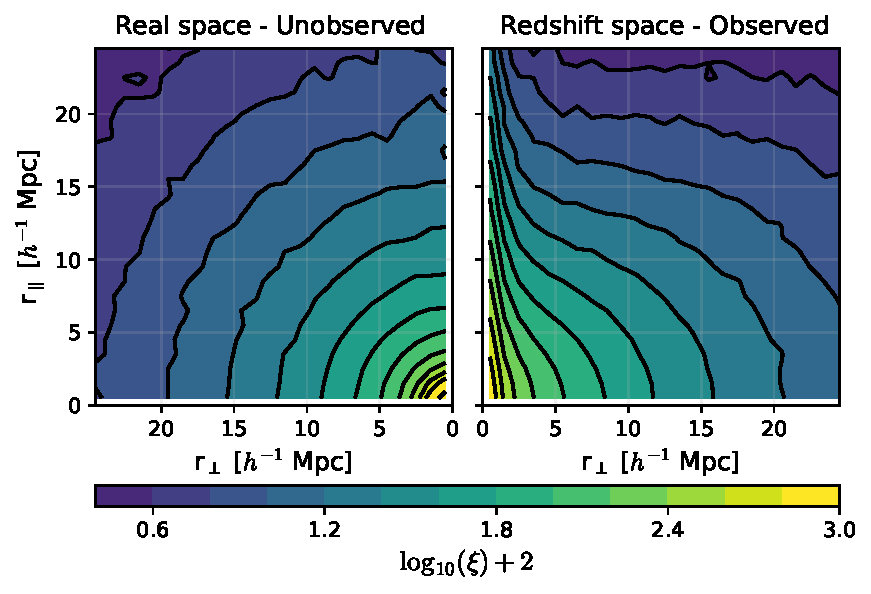
\includegraphics[scale=0.57]{corr_mirror}
		\caption{Correlation function in real-space and redshift-space.}
		\label{fig:mi_corr}
	\end{figure}
	The streaming equation \citep{pe93,fi95, sc04} quantifies the anisotropic correlation function as a convolution of the true isotropic correlation function with the distribution of relative line-of-sight velocities. In the context of the distant observer approximation, it is written as 
	\begin{equation} \label{eq:old_streaming}
	\centering
	1 + \xi_s(s_{\parallel}, s_{\perp}) = \int_{-\infty}^{\infty}  \left[ 1 + \xi_{\mathrm{R}}(r) \right]
	P_{v_{\mathrm{los}}}\left(s_{\parallel} - r_{\parallel} \mid r_{\parallel}, r_{\perp}\right) \dif r_{\parallel} \, ,
	\end{equation}
	where $r = \sqrt{r_{\parallel}^2 + r_{\perp}^2}$ and $v_{\mathrm{los}}$ is the relative line-of-sight velocity. We set the line-of-sight axis along the $z$-axis for the remainder of this paper. The pair weighted quantity, $v_{\mathrm{los}}$, can then be defined as
	\begin{eqnarray}\label{eq:rel_los}
	\centering
	v_{\mathrm{los}} = \left(\mathbf{v}{_2} - \mathbf{v}{_1}\right)\cdot \hat{\mathbf{r}}{_{\mathrm{los}}} = v_{\parallel} \mathrm{sgn}\left(r_{\parallel}\right) \, ,
	\end{eqnarray}
	\noindent where 
	\begin{eqnarray}
	v_{\parallel}= v_{z_2} - v_{z_1} \, , \\
	r_{\parallel}= r_{z_2} - r_{z_1}\, .
	\end{eqnarray}
	
	\subsection{Ingredients}
	
	\begin{figure*}
		\centering
		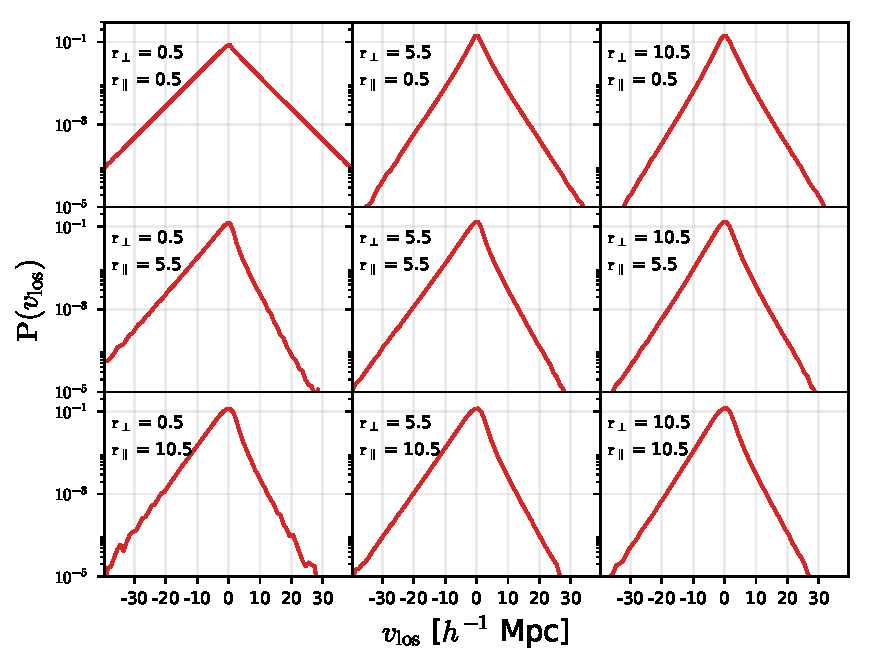
\includegraphics[scale=0.88]{rel_los_grid}
		\caption{Relative line-of-sight velocity distribution. The distance mentioned in each subplot refers to the mean value of each bin, having a bin width of 1 $h^{-1}$ Mpc.}
		\label{fig:rel_los}
	\end{figure*}
	
	In this section, we discuss about the three ingredients (i.e. the 2D anisotropic redshift-space correlation function, 1D isotropic real-space correlation function and the relative line-of-sight velocity distribution) entering the streaming equation. Firstly we turn our focus to the 1D real-space correlation function $\xi_R(r)$. The correlation functions were computed using the Landy-Szalay (LS) estimator \citep{ls93}, which is
	\begin{eqnarray}
	\xi(r) = \frac{DD(r) - 2DR(r) + RR(r)}{RR(r)} \, ,
	\end{eqnarray}
	
	\noindent where $DD(r)$ is the normalised count of galaxy pairs, $DR(r)$ gives the normalised count of pairs given a cross correlation between pairs and random points drawn from a random distribution  and $RR(r)$ is the normalised count of random pairs. In order to mimic the redshift-space distortion effect in the simulation, we displace the position of the particles according to
	\begin{eqnarray}
	\mathbf{s} = \mathbf{x} + \frac{v_z}{aH(a)}\hat{\mathbf{z}} \, ,
	\end{eqnarray}
	\noindent where $a$ is the scale factor and $H(a)$ is the Hubble factor. The ``true'' 2D redshift-space correlation function  is then computed again using LS estimator on these displaced particles.
	
	The relative line-of-sight velocity was measured using Eq.~\ref{eq:rel_los}. For this purpose, we developed a Cython code\footnote{https://github.com/jkuruvilla} which is fully parallelised using MPI. The distribution was calculated from randomly down sampled selection of 256$^3$ particles. The total number of pairs we obtained from this sample is $5.1 \times 10^{11}$ at distances from 0.5 to 100.5 $h^{-1}$ Mpc between the pairs. For the completeness, we have included the periodic boundary conditions while measuring the distance between the pairs. The convergence property of the distribution has been tested with a higher particle number and discussed further in App. \ref{app:conv}. We showcase the relative line-of-sight velocity distribution computed for 256$^3$ particles in Fig.~\ref{fig:rel_los}. One of the immediate conclusion we can draw upon visual inspection is that the distribution changes starkly with the distance and neither an exponential nor a Gaussian will be able to model the distribution accurately. 
	
	To further understand the distribution we try to characterise the distribution using moments. We specifically look into the the first raw moment (mean), the second central moment (variance), the third and the fourth standardised moments (skewness and kurtosis). Fig.~\ref{fig:moments_2d} shows these moments of the relative line-of-sight velocity distribution.. The distribution is marked by non-zero skewness, specifically it is negatively skewed at all the scales shown.  Due to the negative skewness, it can be seen that the mean velocity is negative at most scales. We can interpret this as it is more probable to have in-falling pairs at these scales \citep{sc04}. The distribution showcases a leptokurtic behaviour, implying it has a fatter tail than a normal distribution which has a skewness value of 3.
	
	\begin{figure*}
		\centering
		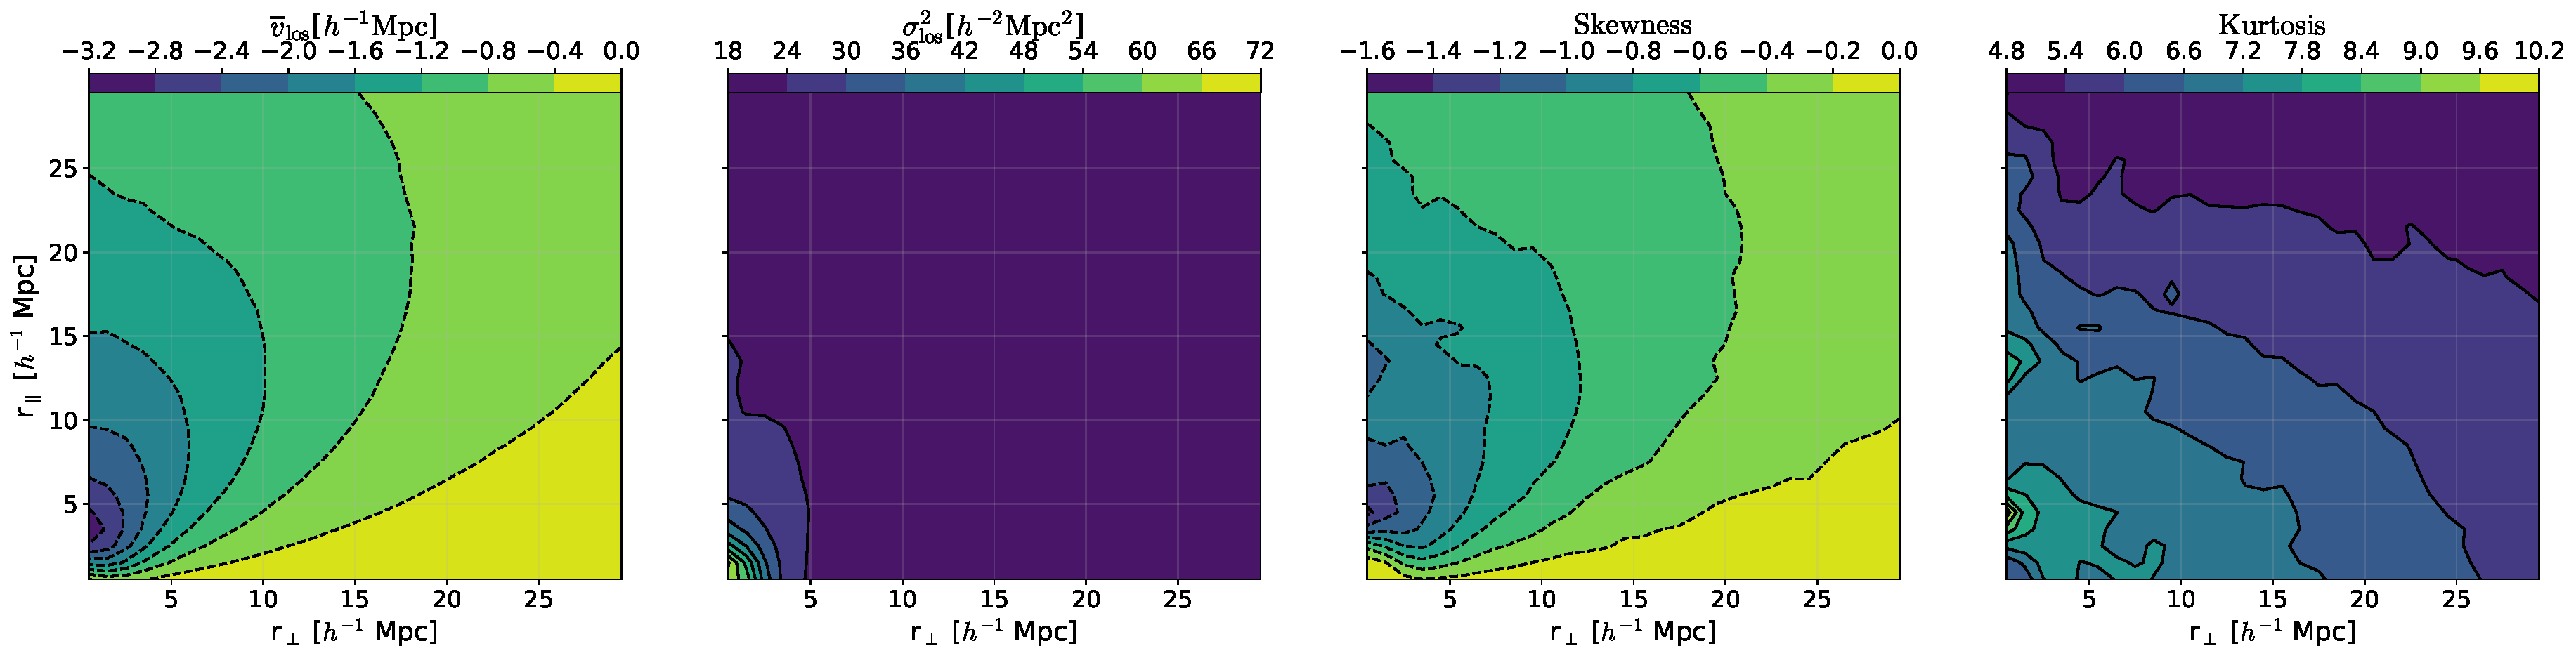
\includegraphics[scale=0.29]{los_moments}
		\caption{Characterising the relative line-of-sight velocity distribution. First panel on left shows the mean relative velocity, followed by the velocity dispersion. The third and the fourth panels shows the standardised moments skewness and kurtosis respectively. Skewness is a measure of the symmetry of the distribution while kurtosis acts as a measure of the tailedness of the distribution.}
		\label{fig:moments_2d}
	\end{figure*}
	
	Having all the ingredients needed, we compute the integral of the streaming equation (Eq.~\ref{eq:old_streaming}) and compare it with the ``true'' redshift-space correlation function measured from the simulations. This is shown in Fig.~\ref{fig:old_str}. It seems that when one checks Eq.~\ref{eq:old_streaming} with simulations there seems to be some discrepancy even though it has been quoted to be exact. The deviation from exactness is worrying as all the phenomenological streaming models are build upon the streaming equation. To understand the discrepancy, we go back to the roots from which we derived the streaming in the next section and try to understand why this deviation from exactness arises.
	
	\begin{figure}
		\centering
		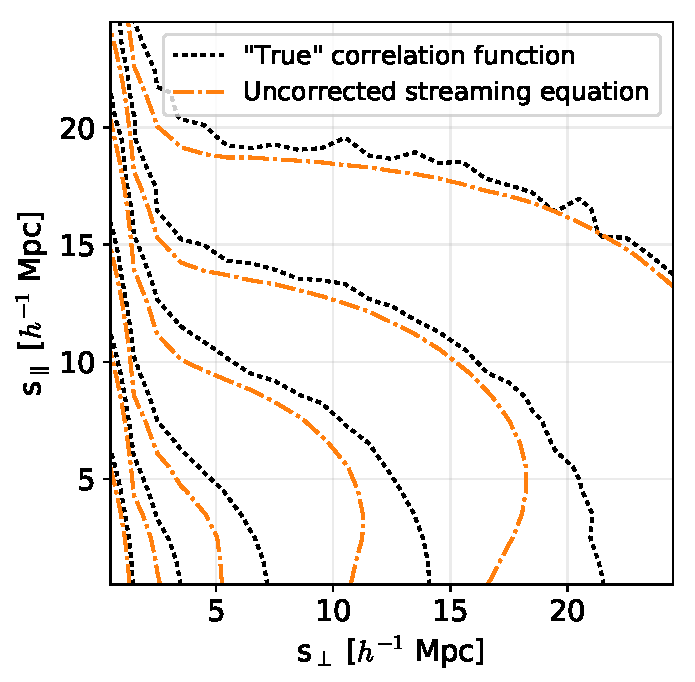
\includegraphics[scale=0.7]{uncorrectedvstrue}
		\caption{When one compares Eq.~\ref{eq:old_streaming} which is quoted as the exact equation against the ``true'' correlation function computed from the simulations, it can be seen that they are not exact. The formalism given in Eq.~\ref{eq:old_streaming} leads to an undermined value.}
		\label{fig:old_str}
	\end{figure}
	
	\section{Corrections to Streaming equation}
	
	Correlation function in redshift space can be defined as the probability to find a pair at parallel and perpendicular to line-of-sight distance ($s_{\parallel}$ and $s_{\perp}$), which is given as 
	\begin{eqnarray} \label{eq:prob_red}	
	\dif P = 2\pi s_{\perp} n \left[ 1+\xi_s(s_{\parallel}, s_{\perp})  \right]\dif s_{\parallel} \dif s_{\perp} \, , 
	\end{eqnarray}
	
	\noindent where $\displaystyle \xi_s(s_{\parallel}, s_{\perp})$ is the 2D anisotropic redshift-space correlation function. This could also written in terms of real space quantities as
	%\noindent The probability to find a pair in redshift space is 
	\begin{multline} \label{eq:prob_real}
	\dif P = 2\pi s_{\perp} n \left[ 1+\xi_{\mathrm{R}}(r) \right] P_{v_{\mathrm{los}}}\left(v_{\mathrm{los}}\mid r_{\parallel}, r_{\perp}\right) \\ 
	\delta_\mathrm{D}\left( \left(s_{\parallel} - r_{\parallel}\right)\mathrm{sgn}\left(r_{\parallel}\right) -v_{\mathrm{los}}\right) \dif r_{\parallel} \dif s_{\parallel} \dif s_{\perp} \dif v_{\mathrm{los}} \, .
	\end{multline}
	
	\noindent where $\displaystyle \xi_{\mathrm{R}}(r)$ is the isotropic real-space correlation function and $\displaystyle  P_{v_{\mathrm{los}}}\left(v_{\mathrm{los}}\mid r_{\parallel}, r_{\perp}\right)$ is the relative line-of-sight velocity distribution function. The term inside the Dirac-delta ensures $\displaystyle s_{\parallel} = r_{\parallel} + v_{\parallel}$, which shows how the pairs are displaced. 
	
	Comparing Equations (\ref{eq:prob_red}) and (\ref{eq:prob_real}), and integrating over $v_{\mathrm{los}}$ and $r_{\parallel}$ eliminates the delta function, one obtains
	\begin{multline} \label{eq:streaming}
	1 + \xi_s(s_{\parallel}, s_{\perp}) = \int_{-\infty}^{\infty}  \left[ 1 + \xi_{\mathrm{R}}(r) \right] \\ 
	P_{v_{\mathrm{los}}}\left(\left(s_{\parallel} - r_{\parallel}\right)\mathrm{sgn}\left(r_{\parallel}\right) \mid r_{\parallel}, r_{\perp}\right) \dif r_{\parallel} \, .
	\end{multline}
	\noindent This is the streaming equation, which is exact in the distant-observer approximation. It is to be noted that Eq.~\ref{eq:streaming} is different to the usual streaming equation as seen in literature till now. We can then proceed to break the integral in the following manner
	\begin{multline} \label{eq:streaming_break}
	1 + \xi_s(s_{\parallel}, s_{\perp}) = \int_{-\infty}^0  \left[ 1 + \xi_{\mathrm{R}}(r) \right] 
	P_{v_{\mathrm{los}}}\left(r_{\parallel} - s_{\parallel} \mid r_{\parallel}, r_{\perp}\right) \dif r_{\parallel} \\
	+ \int_0^{\infty} \left[ 1 + \xi_{\mathrm{R}}(r) \right] 
	P_{v_{\mathrm{los}}}\left(s_{\parallel} - r_{\parallel} \mid r_{\parallel}, r_{\perp}\right) \dif r_{\parallel} \, .
	\end{multline}
	
	\noindent  Fig.~\ref{fig:new_str} shows the corrected streaming equation (Eq.~\ref{eq:streaming_break}) compared with the simulation.
	
	
	\begin{figure}
		\centering
		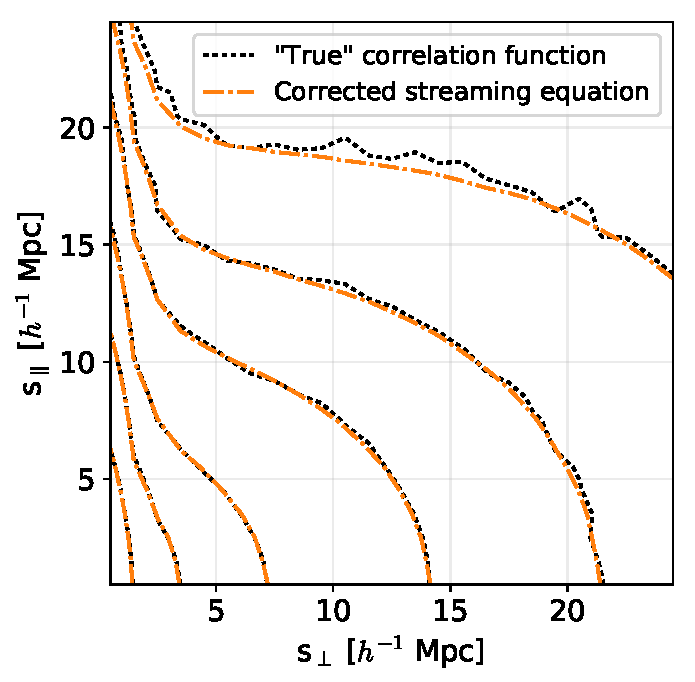
\includegraphics[scale=0.72]{correctedvstrue}
		\caption{Corrected streaming equation compared with the simulation. Orange line denotes the correlation function obtained using the corrected streaming equation(Eq.~\ref{eq:streaming_break}) and black dashed line denotes to the redshift space correlation function measured directly from simulation.}
		\label{fig:new_str}
	\end{figure}
	\begin{figure*}
		\centering
		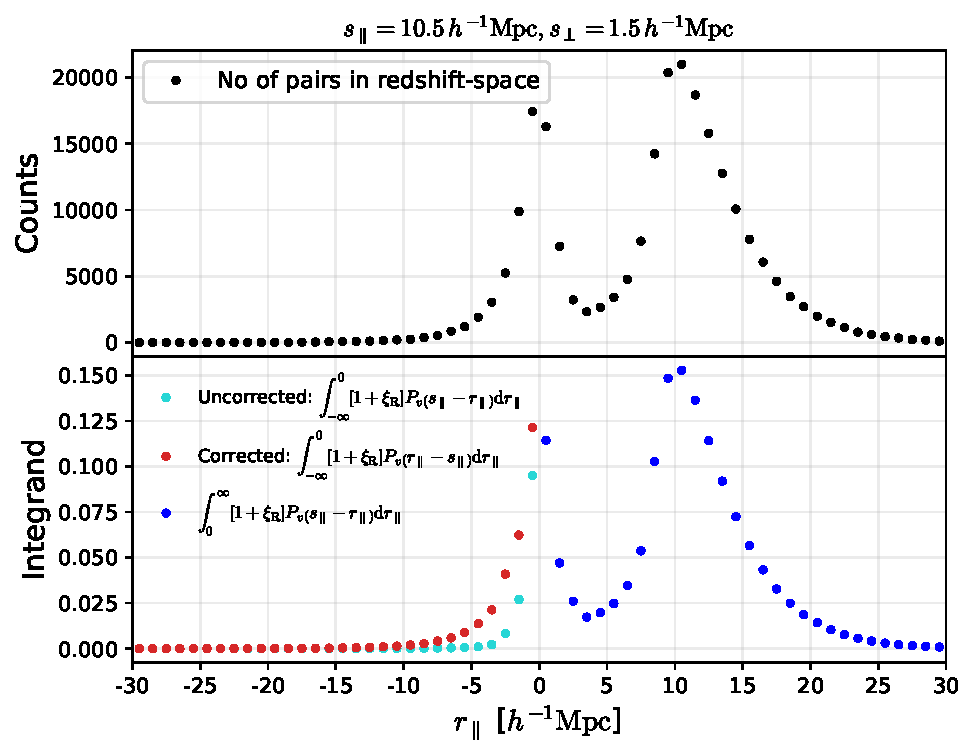
\includegraphics[scale=0.85]{consistency}
		\caption{Consistency check for the streaming equation. Top panel: Shows the number of pairs in redshift-space for particular $s_{\parallel}$ and $s_{\perp}$. $r_{\parallel}$ is obtained as $s_{\parallel} - v_{\parallel}$. Bottom panel: Shows the integrand distribution of the streaming equations at same $s_{\parallel}$ and $s_{\perp}$ as top panel. Due to using the wrong argument of the PDF in the uncorrected integrand, the final value will be undermined compared to the true value.}
		\label{fig:consistency1}
	\end{figure*}
	
	\begin{figure}
		\centering
		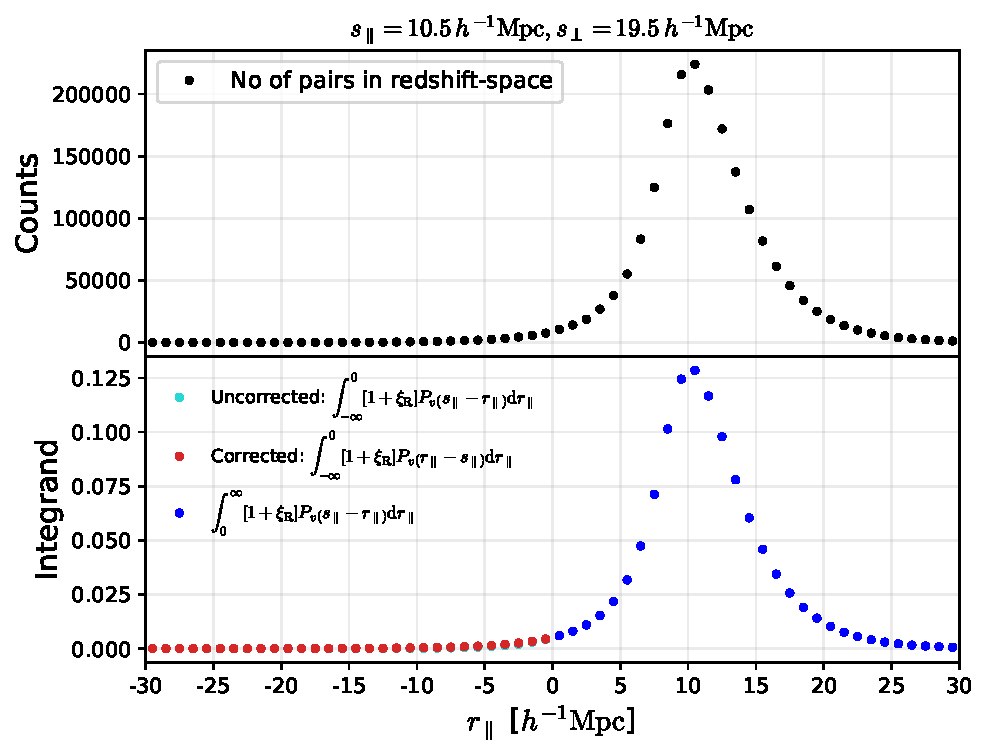
\includegraphics[scale=0.525]{consistency_}
		\caption{Same as Fig.~\ref{fig:consistency1}, but for larger scales. Both the uncorrected (Eq.~\ref{eq:old_streaming}) and corrected (Eq.~\ref{eq:streaming_break}) streaming equations are equivalent at these scales. The impact of pair flips are negligible.}
		\label{fig:consistency2}
	\end{figure}
	
	It is interesting to note that the integral runs from -$\infty$ to +$\infty$. So what does the negative $r_{\parallel}$ mean in the context of streaming model? It means that if we are to take the redshift space to be our reference frame, the negative $r_{\parallel}$ implies pairs which have flipped their position compared to their redshift space counterparts. Fig.~\ref{fig:flip_pairs} clearly demonstrates this where the negative $r_{\parallel}$ is the distance between the pairs which have flipped their position in real-space as compared to the position in redshift-space. This is due to the large relative in-fall velocity of the pairs.It should be noted again that the redshift-space distortions is purely a line-of-sight effect, hence the perpendicular distance between the pairs remains unchanged.
	
	 One can clearly see that with the complete knowledge of the relative line-of-sight velocity distribution and with the correction to account for the pairs which have flipped, we are able to reproduce the true redshift space correlation function accurately. To understand bit more on why there is a need to account for the pair flips and as a consistency check measure, we look at Fig.~\ref{fig:consistency1}. The figure looks at a particular length scale in redshift-space, in this case $s_{\parallel} = 10.5 \,h^{-1}\mathrm{Mpc}$ and $s_{\perp} = 1.5\,h^{-1}\mathrm{Mpc}$. It is quite interesting to note that the plot features two distinct distributions. The first distribution which peaks around $r_{\parallel} = 0$ corresponds to pairs which are in a high density region. These are the pairs which have a large relative velocity and amongst these some undergo pair flips ($r_{\parallel} < 0$). So we can understand that for pairs in a high density region, it is equally likely to undergo pair flips as compared to pairs that do not. The second distribution in the plot peaks around $s_{\parallel} = r_{\parallel}$, these are mainly pairs which are moving away from each other according to Hubble flow (since $v_{\parallel}=0$). In a sense, by looking at the redshift-space distortion effect like this, we are able to disentangle the linear and non-linear effects. To be concise, the distribution around $r_{\parallel} = 0$ is what causes the FoG effect while the distribution around $s_{\parallel} = r_{\parallel}$ causes the Kaiser effect. The bottom panel of Fig.~\ref{fig:consistency1}, shows how the integrand of the streaming equation looks like for a particular length scale in redshift-space. This panel acts as a consistency check and we can understand in a clearer way why the streaming equation would undermine the correlation function if the pair flips are unaccounted for. Due to the asymmetric nature of the velocity distribution, it is essential to pick the argument of the velocity distribution with the right parity. Otherwise we end up neglecting the flipped pairs.
	 
	 We do the same exercise for a larger scale in Fig~\ref{fig:consistency2} and see that both formulations are equivalent since at large scales, we do not expect to see FoG effect and subsequently no pair flips. At these scales we only see one distribution which again peaks around $s_{\parallel} = r_{\parallel}$, telling us that most of the pairs are moving away from each other according to Hubble flow. So we can understand that these corrections are essential if we need to accurately model RSD at scales of $s<20  \,h^{-1}\mathrm{Mpc}$. For large scales, both the formulations will be equivalent.
	 
	\begin{figure}
		\centering
		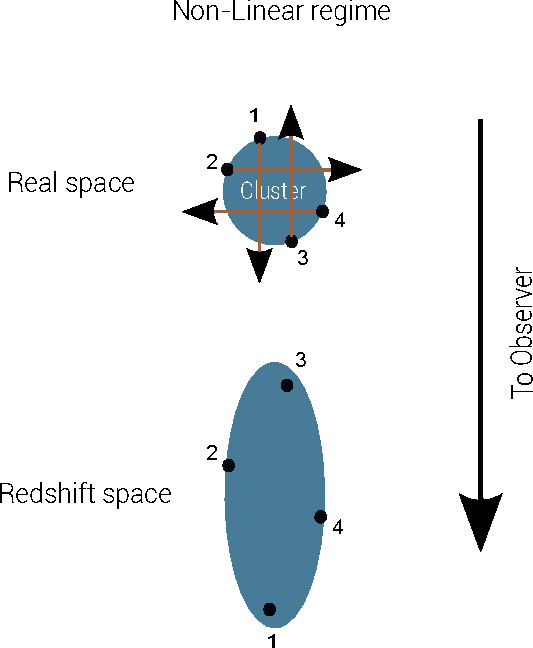
\includegraphics[scale=0.6]{RSD_nonlin1}
		\caption{Pair flips happening due to the ``Finger-of-God'' effect which is a non-linear effect. In this figure, we take the redshift-space as our reference frame. In that framework, objects 1 and 3 here then represent the flipped pairs in real-space. Pair flips are a result of the high relative in-fall velocity of these pairs at non-linear scales.}
		\label{fig:flip_pairs}
	\end{figure}
	
	\subsection{Relation to radial and tangential components of pairwise velocity}
	
	It is of interest to see how the relative line-of-sight velocity is connected to the radial and tangential components of the pairwise velocity. The radial component is defined as the component which is along the separation vector, which can be mathematically written as
	\begin{eqnarray}	
	v_{\mathrm{r}} = \left(\mathbf{v}_2 - \mathbf{v}_1\right)\cdot \hat{\mathbf{r}} \, .
	\end{eqnarray}
	However before we define the tangential component we will need to introduce few other terms as follows
	\begin{eqnarray}
		\mathbf{n}_{12} = \left(\mathbf{r}_2 - \mathbf{r}_1\right) \times \hat{\mathbf{z}} \, ,
	\end{eqnarray}	
	\noindent where $\mathbf{n}_{12}$ is the normal vector to the plane defined by the pairwise vector and the line-of-sight axis, which in this case is the z-axis. 
	\begin{eqnarray}
	v_{\mathrm{away}} = \left(\mathbf{v}_2 - \mathbf{v}_1\right) \cdot \hat{\mathbf{n}}_{12} \, ,
	\end{eqnarray}	
	\noindent where $v_{\mathrm{away}}$ is the velocity component which is in direction of the normal vector away from the plane. Knowing these quantities, we can define the tangential velocity vector as follows
	\begin{eqnarray}
	\mathbf{v}_{\mathrm{t}} = \left(\mathbf{v}_2 - \mathbf{v}_1\right) - (v_{\mathrm{r}}\cdot \hat{\mathbf{r}}) - (v_{\mathrm{away}} \cdot \hat{\mathbf{n}}_{12}) \, .		
	\end{eqnarray}
	\noindent However we are interested in the magnitude of the tangential component which we define as
	\begin{eqnarray}
		v_{\mathrm{T}} = \mathrm{sgn}(v_{t_z})\, \lvert \mathbf{v}_{\mathrm{t}} \rvert \, .
	\end{eqnarray}
	
	 The relative line-of-sight velocity can then be related to the radial and tangential components pairwise velocity as follows
	\begin{eqnarray} \label{eq:los_vel_equivalence}
	v_{\mathrm{los}} = \mathrm{sgn}(r_{\parallel}) \left[v_{\mathrm{r}} \cos\theta + v_{\mathrm{T}}\sin\theta\right] \, ,
	\end{eqnarray}
	\noindent where $\cos\theta = r_{\parallel}/r$. Fig.~\ref{fig:los_relation} shows that the equivalence of Eq.~\ref{eq:los_vel_equivalence} indeed holds true. Thus it is exact. As we know exactly how to go from one formulation to another, it would be interesting to how they are related to each other statistically, namely we show the first three cumulants and how they are related to each other in the coming subsections.

	
	\begin{figure*}
		\centering
		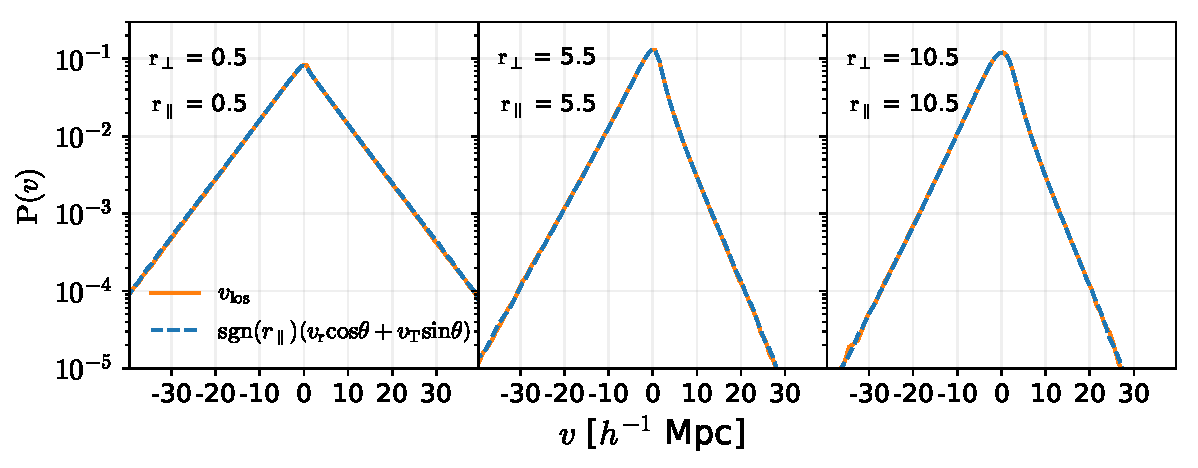
\includegraphics[scale=0.9]{los_velrelation}
		\caption{Shows the equivalence of relative line-of-sight velocity to the radial and the tangential component of the pairwise velocity as given by Eq.~\ref{eq:los_vel_equivalence}.}
		\label{fig:los_relation}
	\end{figure*}
	\subsubsection{First cumulant}
	
	To see how the first cumulant of relative line-of-sight velocity is connected to raw moments of the radial and tangential components, we need to average Eq.~\ref{eq:los_vel_equivalence}. On averaging, we obtain the following 
	\begin{eqnarray}
		\left\langle v_{\mathrm{los}}\right\rangle = \mathrm{sgn}(r_{\parallel}) \left[\left\langle v_{\mathrm{r}}\right\rangle \cos\theta + \langle v_{\mathrm{T}}\rangle\sin\theta\right] \, .
	\end{eqnarray}
	\noindent However due to isotropy $\langle v_{\mathrm{T}}\rangle = 0$, implying the contribution to the mean from the tangential component vanishes. Mean of the relative line-of-sight velocity is then
	\begin{eqnarray}\label{eq:v1}
		\left\langle v_{\mathrm{los}}\right\rangle = \mathrm{sgn}(r_{\parallel}) \left[\left\langle v_{\mathrm{r}}\right\rangle \cos\theta \right] \, .
	\end{eqnarray}	
	
	\noindent The presence of $ \mathrm{sgn}(r_{\parallel}) $ term is essential as it ensures that $\left\langle v_{\mathrm{los}}(-r_{\parallel},r_{\perp})\right\rangle = \left\langle v_{\mathrm{los}}(r_{\parallel},r_{\perp})\right\rangle$, which we have verified from the simulations. In Fig.~\ref{fig:cumulants}, we show the equivalence of Eq.~\ref{eq:v1} and show that they are equivalent.
	\subsubsection{Second cumulant}
	The second cumulant of the relative line-of-sight velocity is related to its raw moments through
	\begin{eqnarray}
		\sigma^2_{\mathrm{los}} =  \left\langle v^2_{\mathrm{los}} \right\rangle - \left\langle v_{\mathrm{los}} \right\rangle^2 
	\end{eqnarray}
	\noindent where we already know the form of $\left\langle v_{\mathrm{los}} \right\rangle$. $\left\langle v^2_{\mathrm{los}} \right\rangle$ can be obtained by first squaring Eq.~\ref{eq:los_vel_equivalence} and then averaging it as below
	\begin{eqnarray}\label{eq:v2}
		\left\langle v^2_{\mathrm{los}} \right\rangle = \left\langle v^2_{\mathrm{r}}\right\rangle \cos^2\theta + \left\langle v^2_{\mathrm{T}}\right\rangle\sin^2\theta \, ,
	\end{eqnarray}
	
	\noindent where we have used $\left\langle v_{\mathrm{r}} v_{\mathrm{T}}\right\rangle$ = 0. This has indeed been checked from the simulation and assured that this condition holds. In fact any term involving averaging of odd power of $v_{\mathrm{T}}$ disappears due to the isotropy.  The second cumulant is then given as 
	\begin{eqnarray}\label{eq:c2}
		\sigma^2_{\mathrm{los}} =  \sigma^2_{\mathrm{r}} \cos^2\theta + \sigma^2_{\mathrm{T}} \sin^2\theta
	\end{eqnarray}
	\noindent where $\sigma^2_{\mathrm{r}} = \left\langle v^2_{\mathrm{r}} \right\rangle - \left\langle v_{\mathrm{r}}\right\rangle^2$ and $\sigma^2_{\mathrm{T}} = \left\langle v^2_{\mathrm{T}} \right\rangle$. We show that the Eq.~\ref{eq:c2} is indeed exact in Fig.~\ref{fig:cumulants}.
	\subsubsection{Third cumulant}
	\noindent The third cumulant of the relative line-of-sight velocity is connected to its raw moments as
	\begin{eqnarray}\label{eq:third_c}
		\gamma_{\mathrm{los}} = & \left\langle v^3_{\mathrm{los}} \right\rangle - 3 \left\langle v^2_{\mathrm{los}} \right\rangle \left\langle v_{\mathrm{los}}\right\rangle  + 2 \left\langle v_{\mathrm{los}}\right\rangle^3 
	\end{eqnarray}
	The form of $\left\langle v^3_{\mathrm{los}} \right\rangle$ can be obtained trivially by cubing Eq.~\ref{eq:los_vel_equivalence} and averaging it thereafter as below
	\begin{eqnarray}\label{eq:v3}
	\left\langle v^3_{\mathrm{los}} \right\rangle = \left\langle v^3_{\mathrm{r}}\right\rangle \cos^3\theta + 3 \left\langle  v_{\mathrm{r}}v^2_{\mathrm{T}}\right\rangle\cos\theta\sin^2\theta \, ,
	\end{eqnarray}	
	\noindent It should be noted that following the isotropy argument again, $\left\langle  v^2_{\mathrm{r}}v_{\mathrm{T}}\right\rangle = \left\langle v^3_{\mathrm{T}}\right\rangle = 0$. This also has been verified from the simulations. Using Eqs.~\ref{eq:v1}, \ref{eq:v2} and \ref{eq:v3}, Eq.~\ref{eq:third_c} can be rewritten as
	\begin{multline}
		\gamma_{\mathrm{los}} = \mathrm{sgn}(r_{\parallel}) \left(\cos^3\theta\left[\left\langle v^3_{\mathrm{r}} \right\rangle - 3 \left\langle v^2_{\mathrm{r}} \right\rangle \left\langle v_{\mathrm{r}}\right\rangle  + 2 \left\langle v_{\mathrm{r}}\right\rangle^3\right] + \right.\\
		\left. 3\cos\theta\sin^2\theta \left[\left\langle  v_{\mathrm{r}}v^2_{\mathrm{T}}\right\rangle - \left\langle  v_{\mathrm{r}}\right\rangle \left\langle v^2_{\mathrm{T}}\right\rangle\right]\right)
	\end{multline}
	\begin{eqnarray}\label{eq:c3}
		\gamma_{\mathrm{los}} = \mathrm{sgn}(r_{\parallel}) \cos\theta \left(\cos^2\theta \,\gamma_{\mathrm{r}} + 3\sin^2\theta \,\mathrm{Cov}\left[v_{\mathrm{r}},v^2_{\mathrm{T}}\right] \right)
	\end{eqnarray}
	\noindent Thus we see that the third cumulant of the relative line-of-sight velocity not only depends on the third cumulant of the radial component of the pairwise velocity but also the covariance between the radial and square of the tangential component of the pairwise velocity. This is similar to the form as mentioned in \citealt{uh15} and \citealt{bi2}, however we have explicitly derived the form and show the equivalence in Fig.~\ref{fig:cumulants}.
	
	\begin{figure*}
	\centering
	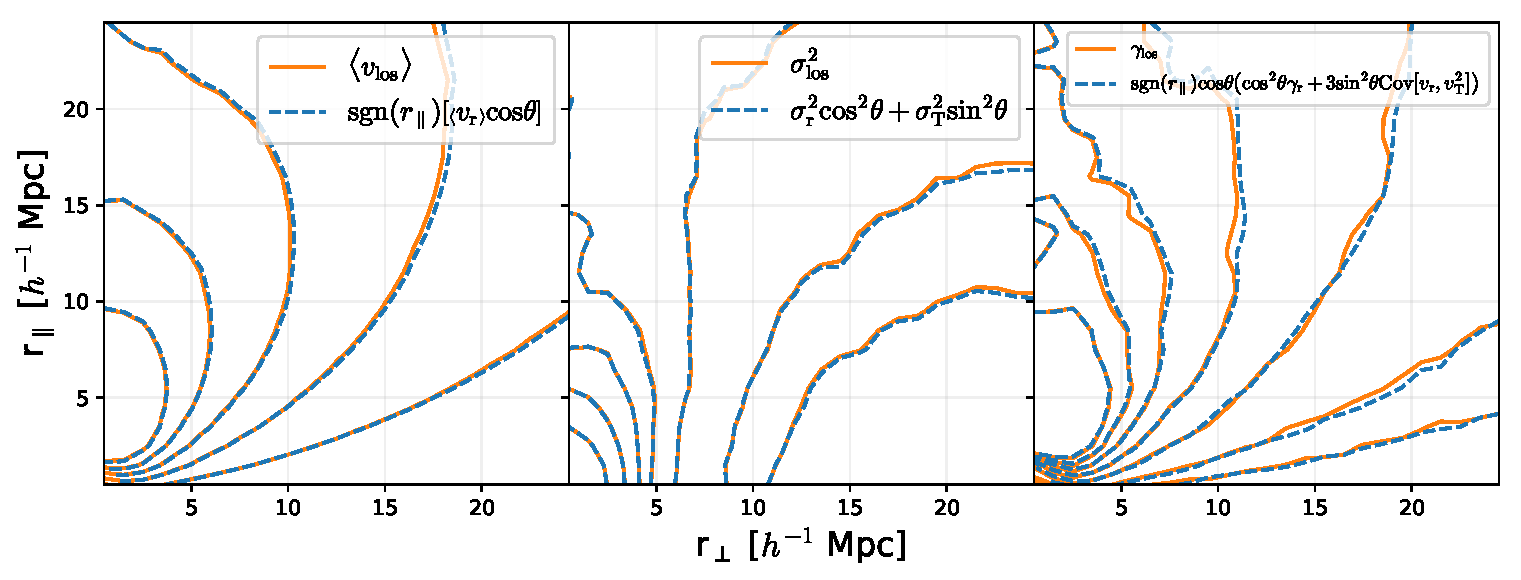
\includegraphics[scale=0.7]{cumulants}
	\caption{Checking the equivalence of the cumulants as shown in Eqs.~\ref{eq:v1}, \ref{eq:c2} and \ref{eq:c3}}
	\label{fig:cumulants}
\end{figure*}
	
	\section{Dissecting Velocity Distribution}
	
	To have a better understanding of the relative line-of-sight velocity distribution, it is important to know how halo and non-halo particles plays a role in the distribution. For this purpose, we classify the dark matter particles as either `halo' particles or `field' particle. This was done with the help of ROCKSTAR halo finder. Particles which were identified to belong to a halo were subsequently classified as `halo' particles and the rest as `field' particles.  
	
	Fig~\ref{fig:rel_los_comp} shows the result of how the components contribute to the total distribution. At the very small scales as seen in the case of mean distance of $r_{\perp} = r_{\parallel} = 0.5 h^{-1}$ Mpc, the distribution is powered by the halo-halo particle pairs. This is not surprising as at these scales, we expect the pairs to be mostly in halos. As the pair separation increases however, the field-field component seems to be the dominant factor especially at the peaks of the distribution. The mean infalling velocity hence seems to be driven by the field-field particle pairs. However it should be noted that halo-halo pairs have a more negative in-fall velocity compared to the field pairs. Narrow wings of the field-field component indicates that the pairs  which does not belong to halos mostly undergo coherent motion. The wings of the total distribution are contributed by both the halo-halo and the field-halo pairs. This clearly shows how the non-Gaussian nature of the relative line-of-sight velocity distribution for the full DM particles arises from the combined effect of the field and halo particles. 
	
	Similarly we can dissect the halo-halo PDF into halo mass subsamples. Fig~\ref{fig:rel_los_mass_comp} shows the contribution from each 
	
	
	\begin{figure*}
		\centering
		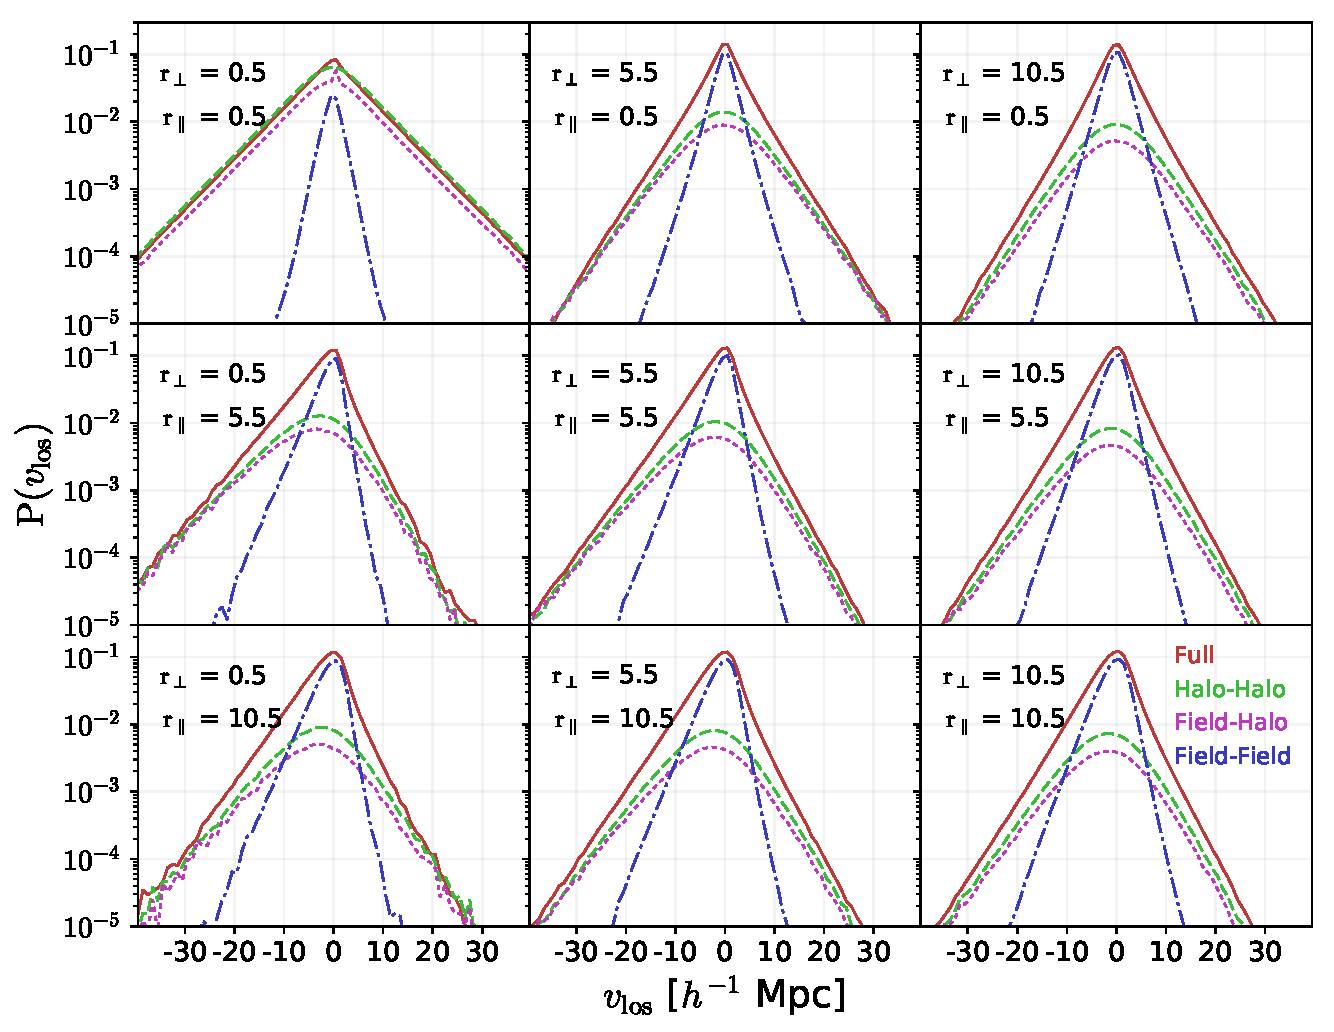
\includegraphics[scale=0.8]{rel_los_components}
		\caption{Relative line-of-sight velocity distribution for different components normalised to full PDF. Green dashed line refers to the pairs which are comprised of 2 halo particles, blue dash dotted line refers to the pair which are formed by 2 field particles and finally magenta dotted line showcases the distribution contributed by pairs in which one of the particle is a field particle and the other a halo particle. The distribution of the full particles is shown using the red solid line. The distance mentioned in each subplot refers to the mean value of each bin, having a bin width of 1 $h^{-1}$ Mpc.}
		\label{fig:rel_los_comp}
	\end{figure*}
	
	
	
	
%	\begin{figure*}
%		\centering
%		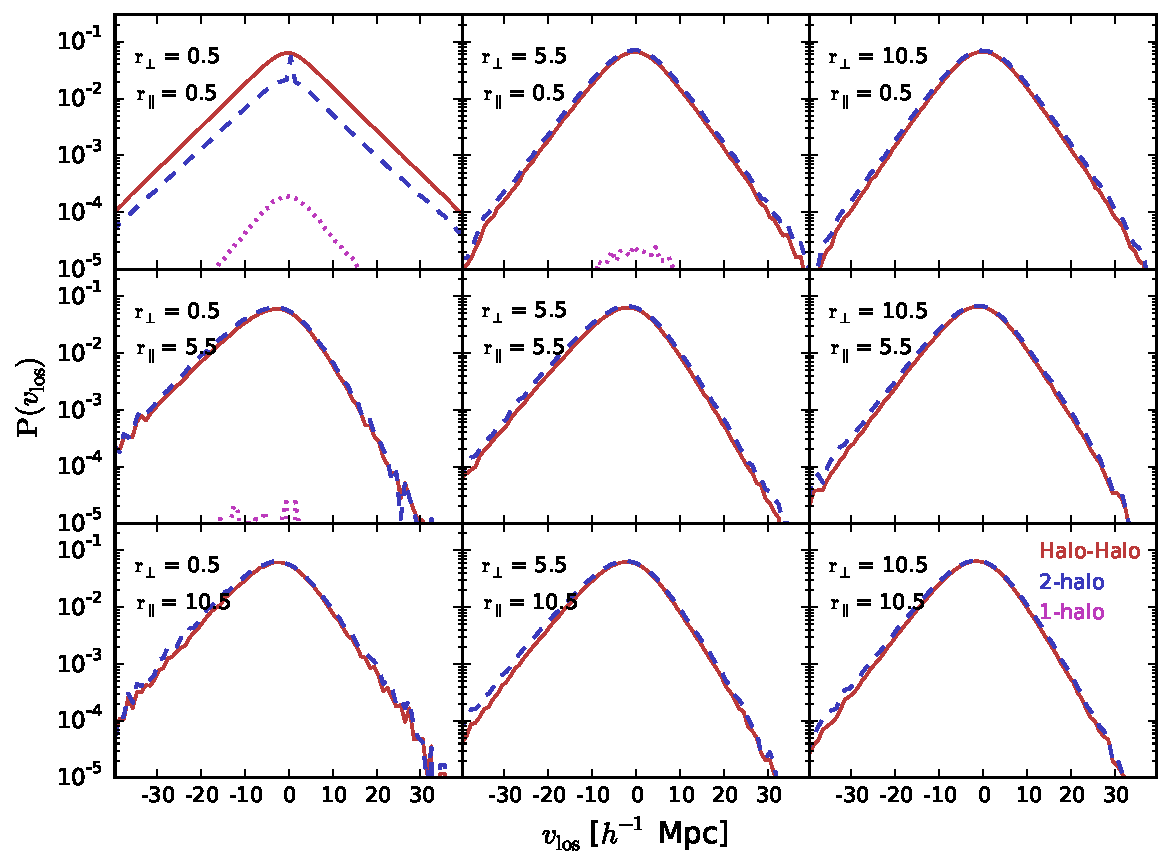
\includegraphics[scale=0.9]{rel_los_halo_components}
%		\caption{Relative line-of-sight velocity distribution for different components. Green dashed line refers to the pairs which are comprised of 2 halo particles, blue dash dotted line refers to the pair which are formed by 2 field particles and finally magenta dotted line showcases the distribution contributed by pairs in which one of the particle is a field particle and the other a halo particle. The distribution of the full particles is shown using the red solid line. The distance mentioned in each subplot refers to the mean value of each bin, having a bin width of 1 $h^{-1}$ Mpc.}
%		\label{fig:rel_los_halo_comp}
%	\end{figure*}
%	
	\begin{figure*}
		\centering
		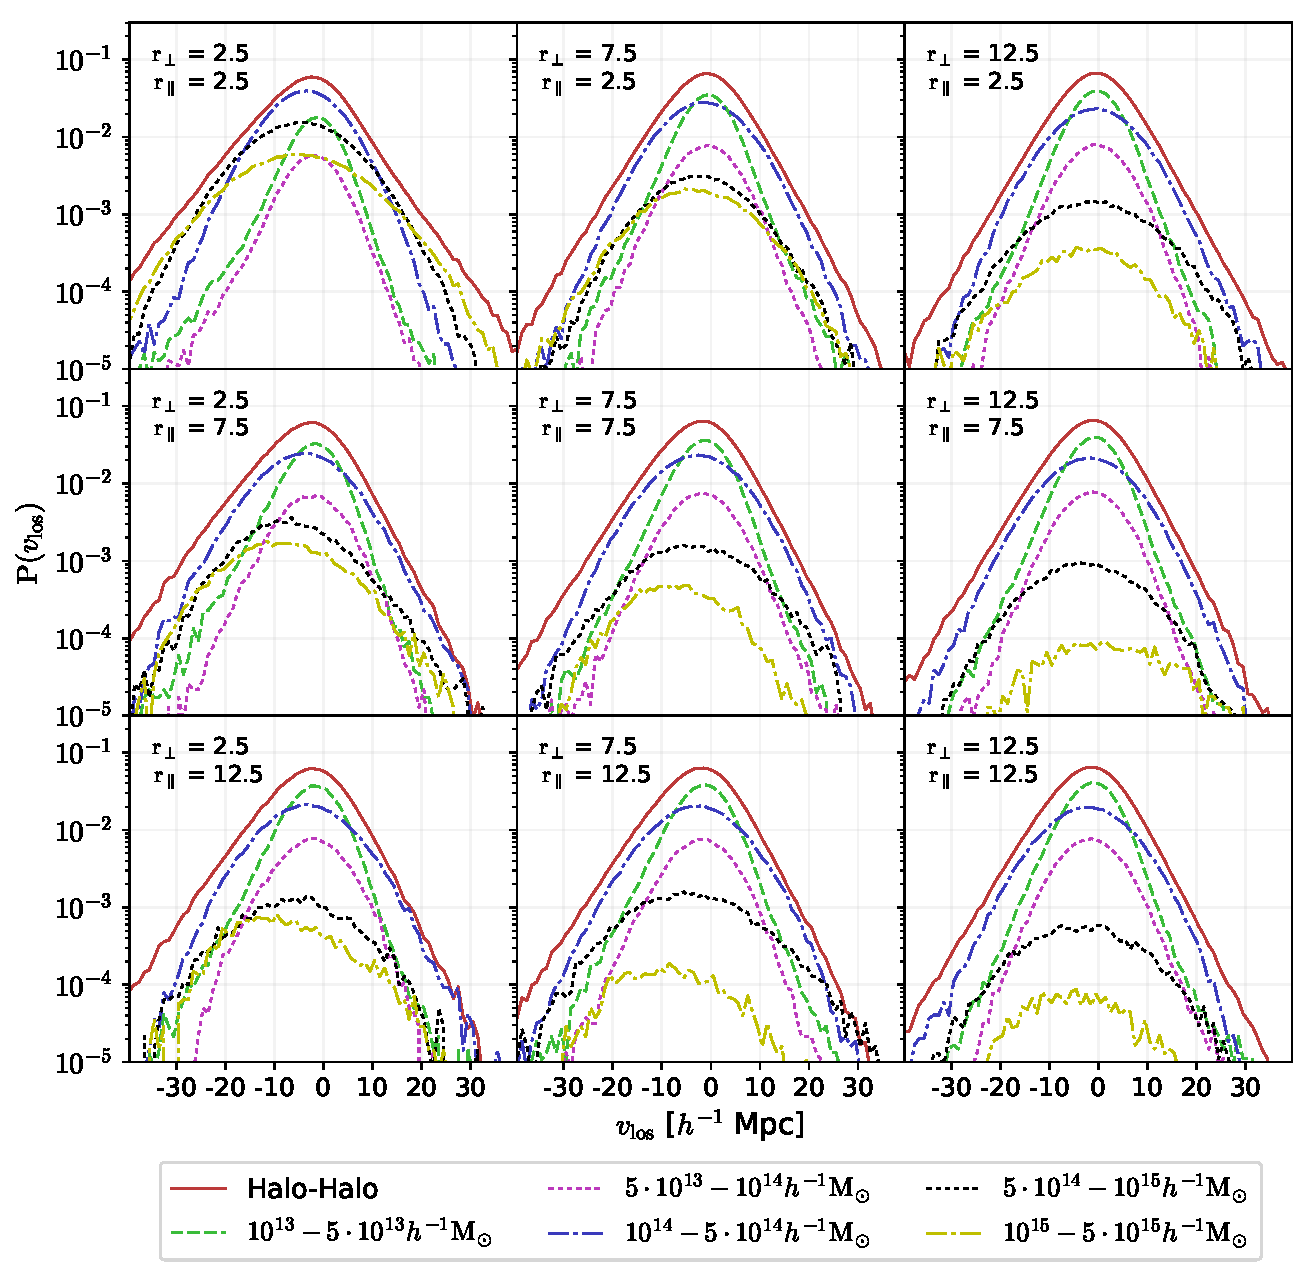
\includegraphics[scale=0.75]{rel_los_mass_components}
		\caption{Relative line-of-sight velocity distribution for different components. Green dashed line refers to the pairs which are comprised of 2 halo particles, blue dash dotted line refers to the pair which are formed by 2 field particles and finally magenta dotted line showcases the distribution contributed by pairs in which one of the particle is a field particle and the other a halo particle. The distribution of the full particles is shown using the red solid line. The distance mentioned in each subplot refers to the mean value of each bin, having a bin width of 1 $h^{-1}$ Mpc.}
		\label{fig:rel_los_mass_comp}
	\end{figure*}

	\section{Phenomenological Model}

	GH is the mixture modelling consisting of normal distribution and Generalised Inverse Gaussian distribution. It is similar to modelling pairwise velocity as mixture of the normal and log-normal density (see tinker). GIG and log-normal are very similar. Try to connect them and see. Density weighted velocity, so would make sense to connect them. Could explain why we use it and why they could be the true distribution.
	
	\section{Conclusions}
	
	
	\section*{Acknowledgements}
	
	JK acknowledges the financial support from the Bonn-Cologne
	Graduate School (BCGS).
	
	%%%%%%%%%%%%%%%%%%%%%%%%%%%%%%%%%%%%%%%%%%%%%%%%%%
	
	%%%%%%%%%%%%%%%%%%%% REFERENCES %%%%%%%%%%%%%%%%%%
	
	% The best way to enter references is to use BibTeX:
	
	\bibliographystyle{mnras}
	\bibliography{str} % if your bibtex file is called example.bib
	
	
	% Alternatively you could enter them by hand, like this:
	% This method is tedious and prone to error if you have lots of references
	% \begin{thebibliography}{99}
	% \bibitem[\protect\citeauthoryear{Author}{2012}]{Author2012}
	% Author A.~N., 2013, Journal of Improbable Astronomy, 1, 1
	% \bibitem[\protect\citeauthoryear{Others}{2013}]{Others2013}
	% Others S., 2012, Journal of Interesting Stuff, 17, 198
	% \end{thebibliography}
	
	%%%%%%%%%%%%%%%%%%%%%%%%%%%%%%%%%%%%%%%%%%%%%%%%%%
	
	%%%%%%%%%%%%%%%%% APPENDICES %%%%%%%%%%%%%%%%%%%%%
	
	\appendix
	
	\section{Convergence}
	\label{app:conv}
	\begin{figure*}
		\centering
		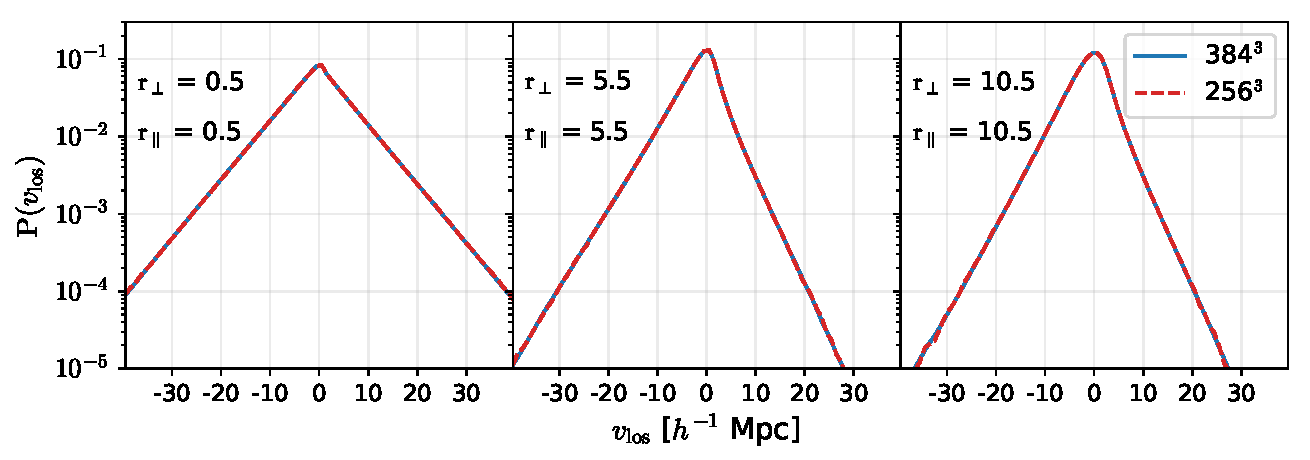
\includegraphics[scale=0.77]{rel_los_convergence}
		\caption{Relative line-of-sight velocity distribution. The distance mentioned in each subplot refers to the mean value of each bin, having a bin width of 1 $h^{-1}$ Mpc.}
		\label{fig:conv}
	\end{figure*}
	
	\section{Extra}
	\label{app:extra}


%%%%%%%%%%%%%%%%%%%%%%%%%%%%%%%%%%%%%%%%%%%%%%%%%%


% Don't change these lines
\bsp	% typesetting comment
\label{lastpage}
\end{document}

% End of mnras_template.tex